\section{系统测试}

软件或硬件的系统测试是在完整的集成系统上进行测试,以评估系统是否符合其指定的要求。通常,系统测试将所有已通过集成测试的软件组件作为其输入,并将软件系统本身与适用的硬件系统集成在一起。集成测试的目的是检测集成在一起的软件单元(称为集合)和硬件之间的任何不一致。系统测试是一种有限的测试类型,它试图检测整个系统内的缺陷。

\subsection{黑盒测试}

黑盒测试是一种软件测试方法,它可以检查应用程序的功能,而无需查看其内部结构或工作情况。这种测试方法可以直接应用在各个级别的软件测试当中:单元测试、集成测试、系统测试和系统验收。所以它有时被称为基于规格的测试。

一般情况下,是不需要应用程序代码/内部结构和编程知识的具体知识的。测试人员知道该软件应该做什么,但不知道它是如何做到的。例如,测试人员知道特定的输入会返回一定的不变的输出,但不知道软件如何产生输出。

为了实现黑盒测试,针对答辩系统编写了测试用例。测试用例是围绕规范和要求构建的,即应用程序应该做什么。测试用例一般都来自于软件的外部描述,包括设计规范、需求要求和设计参数等。虽然使用的测试主要是功能性的,但也可以使用非功能测试。测试设计人员选择有效和无效的输入,并在测试人员的帮助下或者已知结果良好的情况下确定正确的输出,而无需了解测试对象的内部结构。

\subsection{负载压力测试}

负载测试在开发社区中以不同的方式被使用。负载测试通常是指通过模拟多个用户同时访问程序来对软件程序的预期使用效果进行预估。因此,这种测试与多用户系统最相关,例如针对该答辩项目的Web服务器进行的压力测试。最准确的负载测试为模拟实际使用,而不是使用理论或分析建模进行测试。

通过负载测试,我们可以根据实际的客户行为来衡量网站的服务质量(QOS)性能。几乎所有的负载测试工具和框架都遵循经典的负载测试范例:当客户访问您的网站时,脚本记录器记录通信,然后创建相关的交互脚本。负载生成器尝试重放脚本,这些脚本可能在重放时使用不同的测试参数进行调用。在重放过程中,硬件和软件统计数据将被监视和收集,这些统计数据包括物理服务器的CPU、内存、磁盘IO以及响应时间、被测系统(SUT)的吞吐量等,最后综合分析所有这些统计数据,并生成负载测试报告。

在这里,我们不能使用传统的测试工具,比如 ApacheBench(一个单线程命令行计算机程序,用于测量HTTP Web服务器的性能。最初设计用于测试Apache HTTP Server)。因为Meteor代码不会在每个请求上执行,而是首先在浏览器端运行。如果我们发送连续的压力测试请求,将会得到静态的JS代码,这对评估没有意义。

于是在发布到生产环境之前,我们使用MeteorDown为我们的答辩系统进行压力测试。它使用DDP协议与Meteor应用程序进行通信。首先,150行数据被添加到MongoDB的title集合中,每个title文档包含14个字段。在每次测试中,MeteorDown不仅会向用户请求,还会通过Meteor核心提供的方法订阅150行数据。所需的数据量非常大,超出了正常使用的范围。足以反映系统在极高负载下的稳定性。

测试环境的配置信息如表6-1所示,最终的测试结果如图6-1所示。通过测试结果我们可以看到,随着并发数量的增加,虽然单次响应时间逐渐提升,但始终拥令人满意的较高响应速度。每次测试需要与服务器端  Meteor 建立连接,请求并下载数据库中 150 行复杂的 documents。Meteor 可以对这样的测试每分钟运行近万次,并且随着并发数的提高,性能并没有出现明显的下降。这样的性能足以部署在生产环境中,满足大量校园用户在同一时间使用该系统的需求。

\begin{table}
	\centering
	\caption{测试环境配置}  %表格标题
	\begin{tabular}{ll} 
		\hline
		\hline
		核心硬件 & 型号 \\ 
		\hline
		CPU	& Intel Core i7-4700MQ CPU(2.40GHz)\\
		RAM	& DDR3 1600MHz 4Gb*2 \\
		SSD	& PLEXTOR SATA3 PX-128M6M \\
		\hline
		\hline
		核心软件 & 版本 \\ 
		\hline
		OS	& Windows 10 64-bit Professional Edition \\
		MeteorDown & v2.6.0 \\
		Node.js & v4.6.1 \\
		Meteor & v1.4.2 \\
		\hline
	\end{tabular}
\end{table}

\begin{figure}
	\centering
	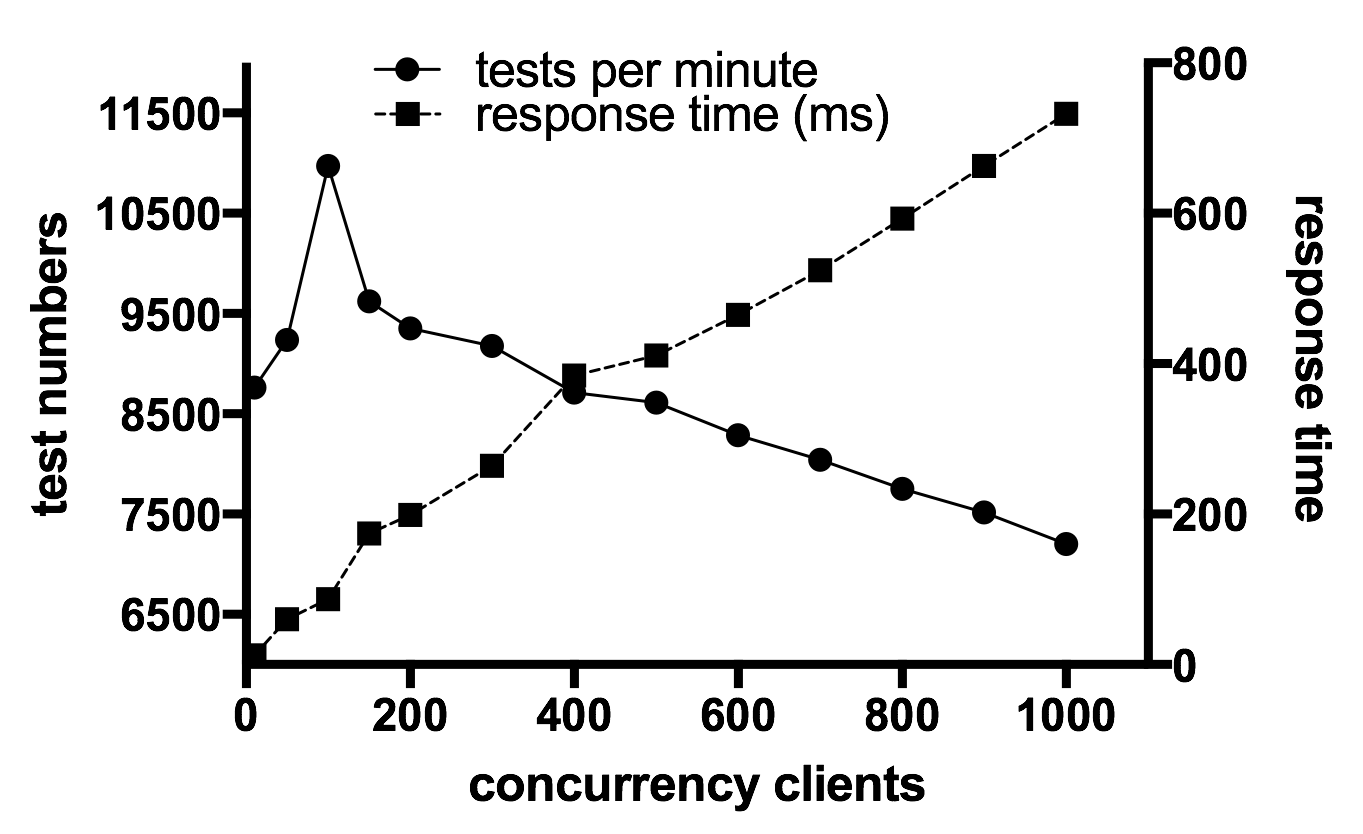
\includegraphics[width=0.7\linewidth]{figure/test_result}
	\caption{压力测试结果}
\end{figure}

负载测试的表现明显超过使用传统后端程序生成 HTML 页面的系统,比如 PHP、ASP.NET 以及 JSP 等编程语言。这这说明服务器端只传输数据,而将数据的渲染交给客户端,能有效降低服务器的运行负载。
